\documentclass{report}

\usepackage{enumerate,fullpage,graphicx,hyperref}
\usepackage{tocloft}

\title{Emergent Architertural Design}
\date{Last edited: \today}
\author{Project members: \\
	\begin{tabular}{c c c}
	\hline 
		Derk-Jan Karrenbeld & 4021967 & 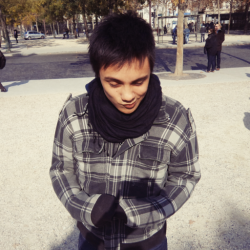
\includegraphics[scale=0.2]{../img/DJ.png}\\ 
		Joost Verdoorn & 1545396 & 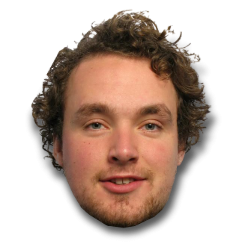
\includegraphics[scale=0.2]{../img/Yoloost.png}\\ 
		Steffan Sluis & 4088816 & 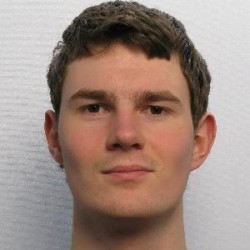
\includegraphics[scale=0.2]{../img/SS.jpeg}\\ 
		Tung Phan & 4004868 & 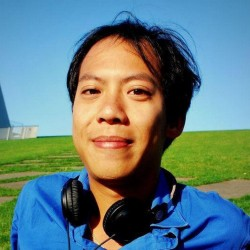
\includegraphics[scale=0.2]{../img/TP.jpeg}\\ 
		Vincent Robbemond & 4174097 & 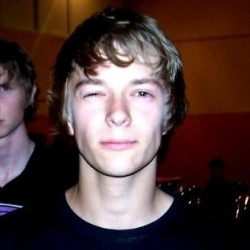
\includegraphics[scale=0.2]{../img/VR.jpeg}\\ 
		\hline 
	\end{tabular} 
	}

\begin{document}
	
	\maketitle

	\setcounter{section}{0}
	\setcounter{secnumdepth}{3}
	\setcounter{tocdepth}{5}
	\renewcommand*\thesection{\arabic{section}}
	
	\pdfbookmark{\contentsname}{toc}
	\tableofcontents

	\clearpage
	
\newcommand{\listfootnotesname}{List of Footnotes}% 'List of Footnotes' title
\newlistof{footnotes}{fnt}{\listfootnotesname}% New 'List of...' for footnotes

\let\oldfootnote\footnote % Save the old \footnote{...} command
\renewcommand\footnote[1]{% Redefine the new footnote to also add 'List of Footnote' entries.
    \refstepcounter{footnotes}% Add and step a reference to the footnote/counter.
    \oldfootnote{#1}% Make a regular footnote.
    \addcontentsline{fnt}{footnotes}{\protect
\numberline{\thefootnotes}#1}% Add the 'List of...' entry.
} 	
	
	\section{Introduction}
		This document contains the architectural design for the application created during the Context Project `Programming Life: Synthetic Biology'. The application is targeted at synthetic biologists and its main purpose is to easily model, simulate and validate the complex workings of a cell. \\
		The design of this application is explained first in terms of its design goals. Then a subsystem decomposition follows, which serves to uncover the inner workings of the application, along with a description of the mapping of subsystems to processes and computers, a hardware/software mapping. After this, the management of data and shared resources is discussed. In conclusion a short summary of the system architecture is given.
		\subsection{Design goals}
			Because the application has a very specific use, modelling cells and the processes within, the main design goal is to make this task as easy and intuitive as possible.
			Further, as requested by the client, we want to give users:
			\begin{itemize}
				\item clear indication that changes can be made and to what these changes apply.
				\item the ability to easily import and export datasets from and to frequently used data-formats e.g. CSV, SBML, HTML, PDF and Excel.
				\item feedback on incomplete/erroneous cell-models created by the user. If mistakes are made, they need to be easily identified and corrected.
				\item compare simulations by plotting data on other simulations.
				\item the ability to work locally without the need to be connected to the server.
				\item feedback on and the ability to share what is saved.
				\item an easy way to undo changes.
			\end{itemize}
			To broaden their knowledge and expand their experience, the developers agreed to use programming languages and frameworks previously unknown to them.
	\clearpage
	\section{Architecture}
	
			\subsection{Overview}
				
			
			\subsection{Server}
				The server subsystems consist of two key parts: the server back end and the database, this can be seen in figure 1. The server keeps an up-to-date copy of the database and sychronises with the client side when possible. In the future it could be used to do calculations that are too complicated for the client-side of the application (calculations are deemed too complicated when they take a notable amount of time to complete).
				The database is used for storage of user data, modules for cell design, as well as cell models created using the application. It provides a centralised storage, so users can share their modelled cells and can access their data anywhere. However the client-side application can function on any platform without a persistent internet connection.
				\clearpage
				\begin{figure}[htb]
				\begin{center}
				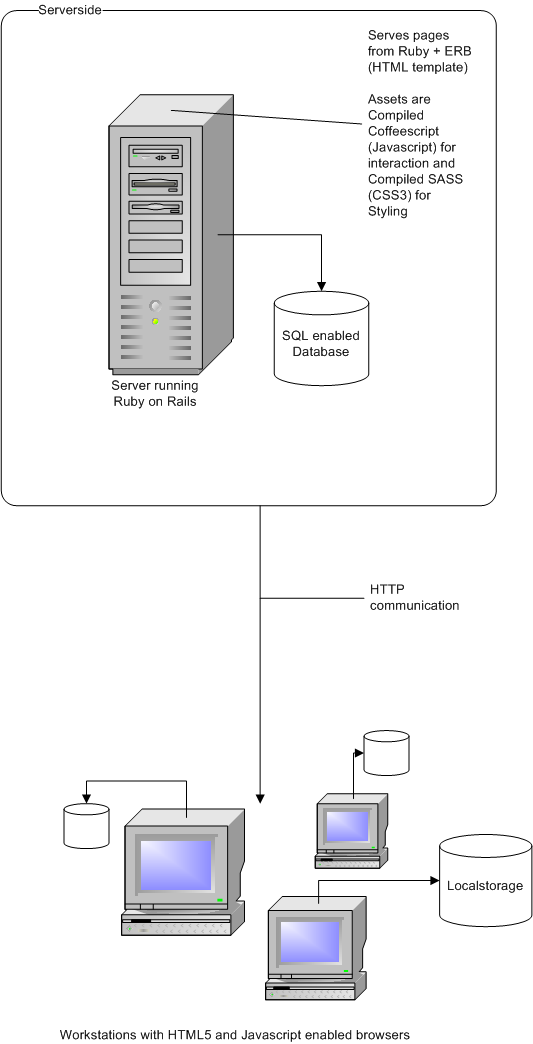
\includegraphics[scale=0.95]{EAD.png}
				\caption{Deployment Diagram}
				\label{fig: EAD}
				\end{center}
				\end{figure}
				\clearpage
									
				\subsubsection{Rails}
					The server runs on Ruby on Rails \footnote{http://api.rubyonrails.org/} . This is a fairly new but very stable platform that is not only free but also open source. This means active development by a lot of people. Problems are easily fixed and this should ease the use of the application that is being designed. The language itself is written from a standpoint where you should just be able to write code and not worry about breaking the interpreter \footnote{www.artima.com/intv/rubyP.html} . This makes it easy to write comprehensible code that executes complex tasks.				
				\subsubsection{MVC}
					The pages served are HTML5 for markup with CSS3 for styling and Javascript for interaction. Pages are built by a comprehensive and solid Model-Viewer-Controller system. This keeps data separated from the representation, further increasing maintainability. Interaction is illustrated in figure 2. Because interaction and data are separated, change of the data through interaction can easily be stored and reversed providing the undo-functionality as per the design goals.			
				\subsubsection{Models and Database}
					Ruby models are mapped to any Relational Database Management System (RDMS \footnote{http://en.wikipedia.org/wiki/Relational\_database\_management\_system} ) such as SQLite, MySQL and PostgreSQL. By not restricting the server database technology, switching systems, servers or extending  their capacity should be fairly simple and easy.
				\subsubsection{Views and ERB} 
					The views are in ERB \footnote{http://ruby-doc.org/stdlib-2.0/libdoc/erb/rdoc/ERB.html} which is an HTML template system. It comes with the Rails framework, so it does not require any extra software. Rails controllers written in Ruby can expose data to these views. New views are easily added this way, so new ways of data representation are quickly devised.
			\clearpage
			\begin{figure}[htb]
				\begin{center}
				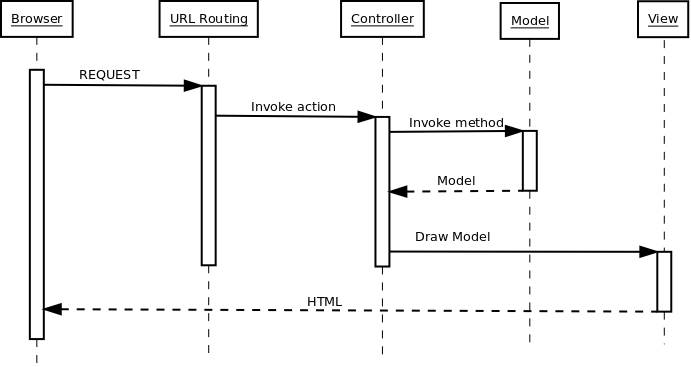
\includegraphics[scale=0.4]{SequenceDiagramLife.png}
				\caption{Sequence Diagram}
				\label{fig: SequenceDiagram}
				\end{center}
				\end{figure}	
			\clearpage

			\subsection{Client}
				The client-side subsystems contain most of the applications functionality. These subsystems are responsible for displaying the graphical environment with all its modules, as well as solving the basic equations.  The client-side subsystems functions independently of the server. Local storage is used as temporary storage when there is no connection to the server. Only the sharing of data and generating reports of cells and their simulation is then not available.
				\subsubsection{Local storage}
					Javascript determines the local storage engine that is availabe and uses that to maintain an offline copy of the application and the created cells/modules. This makes it very easy to design new cells or edit saved cells even when the user isn't connected to the internet. This is communicated to the user, but requires no further interaction. Synchronization is completely transparent.
				\subsubsection{Interaction by Javascript}
					Javascript facilitates interaction and processes all the differential equations. It generates the graphs and the reports with the help of the canvas element and SVG, part of HTML5.
		
		\subsection{Data management}
			When the user has access to the server, it can export simulation results to a report in multiple standardised format, such as \emph{HTML}, \emph{Excel} and \emph{PDF} which can then be shared. Maintaining a standardised format allows for consistency in the reports as requested by the user.		
	
		\subsection{Concurrency}
			Each client runs independently and uses asynchronous communication with the server through \emph{REST}/\emph{CRUD} and \emph{AJAX}. Because of this, concurrency issues are very improbable. The client-side application is web-based, and uses only one process. Shared resources are retrieved atomically from and synchronised atomically with the database. Upon failure, the user is notified and possible solutions are provided. At this point the system does not allow concurrent edits on the same data, but this functionality was not reuqested by the user. Such functionality could be added in the future.\\		
			
	\clearpage
	\section{Software architecture views}
		This section contains all the information about the software architecture of the application. The section is divided into several subsections to group together interesting information and improve readability.	
		
		\subsection{Framework and Development}
			This section describes the key technologies used during a release cycle.
			It is divided into three subsections; development, testing and production.
			The first subsection is about the development phase, where features are realised.
			The second section is about the testing phase, in which the features mentioned before are tested.
			The third section describes the production/release phase, in which a tested feature is implemented.
			
			\subsubsection{Development}
				During development we are making use of Coffeescript \footnote{http://coffeescript.org/\#language} for writing interaction assets, SASS \footnote{http://sass-lang.com/docs/yardoc/file.SASS\_REFERENCE.html} for styling and SVG \footnote{http://www.w3.org/Graphics/SVG/} with the Raphael \footnote{http://raphaeljs.com/reference.html} framework for visualising part of the application.
				Coffeescript and SASS are preprocessors for respectively Javascript and CSS. Using these preprocessors gives us the advantage of cleaner syntax.
				By making use of SVG to render the cell every graphical object is also a DOM object, this enables us to attach Javascript event handlers and modify the objects itself.
				
			\subsubsection{Testing}
				We test the application in a Behaviour Driven Development (BDD \footnote{http://en.wikipedia.org/wiki/Behavior\-driven\_development} ) and Test Driven Development (TDD \footnote{http://en.wikipedia.org/wiki/Test\-driven\_development} ) way. 
				The Javascript assets are tested using the Jasmine framework \footnote{http://pivotal.github.io/jasmine/} . 
				To run all tests in the browser we are making use of the Teabag framework \footnote{https://github.com/modeset/teabag} . 
				To keep track of code coverage we are making use of the Istanbul framework \footnote{https://github.com/gotwarlost/istanbul} .
				The Ruby assets (database, MVC architecture - models, controllers, views - and Rails) are tested using the Rspec framework \footnote{http://rubydoc.info/gems/rspec\-rails/frames} .  
				All tests run automatically using Continuous Integration, a practice in which tests are ran every time work has been done within critical sections of the code. 
				Tests and coverage are used to ensure maintainability, consistency and quality of the code.
				
			\subsubsection{Release}
				During the Production release the Coffeescript assets are compiled to Javascript \footnote{https://developer.mozilla.org/en-US/docs/JavaScript/Reference} and the SASS assets are compiled to CSS, after which they are minified and bundled using uglifier \footnote{http://rubydoc.info/gems/uglifier/2.1.0/frames} . Minified assets take up less space and increase page performance which results in a better user experience and less demand on the web server. 
				SVG is still used for creating visualisations of the cell models.
		\newpage		
		\subsection{Ordinary Differential Equation Solver}
			All computations run client-side and are performed by our ODE Solver, which is built upon the numericjs \footnote{http://www.numericjs.com/} library. This is a library which makes it possible to perform sophisticated numerical computations in pure JavaScript and thus is able to run in the browser. The ODEs are solved using the Dormand-Prince RK method \footnote{http://en.wikipedia.org/wiki/Dormand\%E2\%80\%93Prince\_method} , also known as the ode45-function in MATLAB (previously used by our client).
			
		\subsection{API}
			The API can be found online here: \url{http://coffeedoc.info/github/Derkje-J/programming-life/develop/} \\
			In the future there will be a Rubydoc online for server-side assets and is updated after each commit.
		\newpage
			
	\section{Summary}
		The application is a lightweight, cross-platform graphical design tool with a centralised storage database. The architecture ensures its functionality on different kinds of machines as well as the ease of simulating complex cell models. It not only offers stability, ease and intuitive design, it offers it on every modern machine. During development of this application the design goals are continuously used as a mandate for the functionality and dictates the production flow.
	\section{Glossary}
		This section explains any and all terms that may be ambiguous or unclear:\\
		
		\textbf{REST}: Representational State Transfer, or REST, is an architectural style of large-scale networked software that takes advantage of the technologies and protocols of the World Wide Web. \\
See \href{http://goo.gl/Lfwhs}{http://goo.gl/Lfwhs} for more information.



\listoffootnotes \clearpage

\end{document}
